\documentclass[a4paper,11pt]{article}
%@@@@@@@@@@@@@@@@@@@@@@@@@@@@@@@@@@@@@@@@@@@@@@@@@@@@@@@@@@@
%@@@@@@@@@@@@@@@@      PACOTES BÁSICOS		     @@@@@@@@@@
%@@@@@@@@@@@@@@@@@@@@@@@@@@@@@@@@@@@@@@@@@@@@@@@@@@@@@@@@@@@

\usepackage[T1]{fontenc}
\usepackage[utf8]{inputenc}
\usepackage{lmodern} 
\usepackage[portuguese]{babel}
\usepackage{amsmath}
\usepackage{array}
\usepackage{graphicx}				%para imagens
\usepackage{epstopdf} 				%resolve problemas eps-pdf
\usepackage{pict2e}				%%writting to images
%@@@@@@@@@@@@@@@@@@@@@@@@@@@@@@@@@@@@@@@@@@@@@@@@@@@@@@@@@@@
%@@@@@@@@@@@@@@@@     PACOTES NÃO TAOBÁSICOS		 @@@@@@@@@@
%@@@@@@@@@@@@@@@@@@@@@@@@@@@@@@@@@@@@@@@@@@@@@@@@@@@@@@@@@@@
\usepackage{fancyhdr}				% para o cabeçalho bonito
\usepackage{caption}					%para legendas
\usepackage{subcaption}				% e sublegendas
\usepackage{placeins} 				%controlar o lugar dos floats
\pagestyle{fancy} 					% número de pag e cabeçalho
\usepackage{txfonts} 				%fontes bonitas? acho que para o título
\usepackage[usenames]{color} 		% algo com gunplot e eps
\usepackage{ifthen}
\usepackage{xparse}
\graphicspath{{./../images/}{./../data/}{./graph/}}	% procura imagens nessa pasta
\usepackage{float} %%para definir ambiente gráfico
\newfloat{Gráfico}{hbtp}{lop}[section]
%\usepackage{undertilde}	%%para notação de vetor do yuri
\usepackage[import]{xy} % para escrever em imagens
\xyoption{import}

\usepackage{listings}
\lstset{frame=single,}
%@@@@@@@@@@@@@@@@@@@@@@@@@@@@@@@@@@@@@@@@@@@@@@@@@@@@@@@@@@@
%@@@@@@@@@@@@@@@@      Cabeçalho de cada página      @@@@@@@
%@@@@@@@@@@@@@@@@@@@@@@@@@@@@@@@@@@@@@@@@@@@@@@@@@@@@@@@@@@@
\setlength{\headheight}{25pt}%compila sem erro
	\fancyhead{}
	\fancyfoot{}
	\fancyhead[R]{Sistemas de Medição}%direito superior
	\fancyhead[L]{
\includegraphics[height=0.25in]{./../images/logo_unb.pdf}}%esquerda superior
	\fancyfoot[C]{\thepage}%baixo centro
%E: Even page, O: Odd page, L: Left field, C: Center field, R: Right field, H: Header, F: Footer
% em documentos com dois lados use LO, RO. como esse documento não tem lados essa opção é inútil


%@@@@@@@@@@@@@@@@@@@@@@@@@@@@@@@@@@@@@@@@@@@@@@@@@@@@@@@@@@@
%@@@@@@@@@@@@@@@@      NOVOS COMANDOS		      @@@@@@@@@
%@@@@@@@@@@@@@@@@@@@@@@@@@@@@@@@@@@@@@@@@@@@@@@@@@@@@@@@@@@@
\newcommand\undermat[2]
	{
	  \makebox[0pt][l]
	  	{$\smash{\underbrace{\phantom{%
    \begin{matrix}#2\end{matrix}}}_{\text{$#1$}}}$
    		}#2
    	}
    	
\newcommand{\HRule}
	{
	\rule{\linewidth}{0.5mm}
	}
	
\newcommand{\EmptyPage}
	{
	\thispagestyle{empty}
	\mbox{ }
	\newpage	
	} 
	
\newcommand{\MakeMyTitlePage}[4]
%%Argumentos: 
%1º Nome da Matéria
%2º subtítulo ex: experimento IV
%3º título
%4º autores
% exemplo de autores:
%	\begin{center} \large
%		\begin{tabular}{llr} \
%		& & \\[0.05cm]		
%		Professora & Nadia Maria de Liz Koche & \\
%		
%		Alunos:& & \\
%		& Juarez A.S.F 					& 11/0032829\\
%		& Sérgio Fernandes da Silva Reis & 11/0140257\\
%		& Jedhai Pimentel				& 09/0007883\\	[0.05cm]	
%		\end{tabular}
%	\end{center}
{
\begin{titlepage}
\begin{center}

% Upper part of the page. The '~' is needed because \\
% only works if a paragraph has started.

\includegraphics[width=\textwidth]{./../images/logo_unb.pdf}~\\[1cm]

\Huge #1\\[0.5cm]

\huge #2

% Title
\HRule \\[0.4cm]
{ \huge \bfseries  #3}\\[0.4cm]

\HRule \\[0.5cm]

{\large \today}


\vfill %%o que vier depois vai ao fim da páginda


%Autor e Professor
\begin{center} \large
#4
\end{center}

\end{center}
\end{titlepage}

\EmptyPage
\tableofcontents
\newpage

}
	
%@@@@@@@@@@@@@@@@@@@@@@@@@@@@@@@@@@@@@@@@@@@@@@@@@@@@@@@@@@@
%@@@@@@@@@@@@@@@@      NOVOS AMBIENTES		      @@@@@@@@@
%@@@@@@@@@@@@@@@@@@@@@@@@@@@@@@@@@@@@@@@@@@@@@@@@@@@@@@@@@@@
\newcounter{graph-c}
\setcounter{graph-c}{0}


%\NewDocumentEnvironment{Graph}{m}
 % {%antes
  %\addtocounter{graph-c}{1}
  %\begin{figure}
  %}
 %{
 %depois
%	\end{figure} 
%	\caption*{Grafico \arabic{graph-c} - #1}
 %}

















%inclui todosos pacotes utilizados

\newcommand{\MyBox}[1]
{
	\begin{tabular}{|l|}\hline
	  #1 \\ \hline	    
	\end{tabular} 	
}

\lstset{frame=single,}	

\begin{document}



\MakeMyTitlePage
{Análise Dinâmica Linear}
{Experimento IV}
{Identificação das Plantas Servo por meio
da Análise da Resposta Temporal}
{%autores
		\begin{tabular}{llr} \
		& & \\[0.05cm]		
		Professor & Henrique Cezar Ferreira & \\
		
		Alunos:& & \\
		& Juarez A.S.F 												& 11/0032829\\
		& Luís Henrique Vieira Amaral						&	10/0130488 	
			\end{tabular}
}

%@@@@@@@@@@@@@@@@@@@@@@@@@@@@@@@@@@@@@@@@@@@
%@@@@@@@@@@@@@@@@      OBJETIVOS      @@@@@@@@@@@@@@@@@@
%@@@@@@@@@@@@@@@@@@@@@@@@@@@@@@@@@@@@@@@@@@@
\section{Objetivos}
\paragraph{} Obter a função de transferência da planta servo rotacional em estudo
a partir da análise da resposta temporal.
%@@@@@@@@@@@@@@@@@@@@@@@@@@@@@@@@@@@@@@@@@@@@@
%@@@@@@@@@@@@@@        INTRODUÇÃO       @@@@@@@@@@@@@@@@@@@@ 
%@@@@@@@@@@@@@@@@@@@@@@@@@@@@@@@@@@@@@@@@@@@@@
\section{Introdução Teórica}
\paragraph{} Se conhecermos a forma esperada da função de transferência
de um sistema, podemos estimar os parâmetros desta por meio da análise
do gráfico da resposta no tempo. Para a planta rotacional em estudo
esperamos uma função
de transferência na forma:
\begin{equation}
 \frac{\Omega _l (s)}{V_m(s)} = \frac{K}{\tau s + 1}
\end{equation}

em que $\Omega_l(s)$ é a transformada de Laplace da velocidade 
angular do eixo de carga, $V_m$ a transformada do sinal de tensão 
aplicado no motor, K o ganho em regime estacionário e $\tau$ a 
constante de tempo. 

\paragraph{} O sinal aplicado é o degrau de amplitude A. A 
transformada de Laplace desse sinal é:

\begin{equation}
  V_m(s) = \frac{A}{s}
\end{equation}
ao multiplicarmos pela função de transferência temos a saída em 
Laplace:

\begin{equation}
 \Omega _l(s) = \frac{A}{s} \cdot \frac{K}{\tau s + 1} = 
  A \cdot k \cdot (\frac{1}{s} - \frac{1}{s + \frac{1}{\tau}})
\end{equation}
aplicando a transformada inversa obtemos a resposta no tempo:

\begin{equation}
 v(s) = A \cdot k \cdot(1 - e^{-\frac{t}{\tau}})
\end{equation}

de onde vemos que :
\begin{equation}
  \begin{array}{l}
  \mbox{(valor final)} V_f = A \cdot k \\
  \frac{d}{dt}(v(t))|_{t = 0} = \frac{A \cdot k}{\tau}
  \end{array}
  \label{eq:leEq}
\end{equation}

vemos então que a partir da inclinação inicial da reta tangente e 
do valor final da resposta ao degrau os parâmetros estão 
completamente determinados.

%@@@@@@@@@@@@@@@@@@@@@@@@@@@@@@@@@@@@@@@@@@@
%@@@@@@@@@@@@       PROCEDIMENTOS        @@@@@@@@@@@@@@@@@@
%@@@@@@@@@@@@@@@@@@@@@@@@@@@@@@@@@@@@@@@@@@@
\section{Descrição Experimental}
\begin{itemize}
 \item
Iniciou-se o experimento abrindo o modelo identifica\_SRV02.mdl 
no software Simulink. Ao abrir o modelo observou-se três subsistemas 
distintos: um que representava o modelo real, um obtido através de 
cálculos e outro obtido, posteriormente, experimentalmente. Como 
entrada havia disponível excitação degrau ou uma onda quadrada, ao 
final dos blocos os dados obtidos era enviados para a sessão workload 
do MATLAB. Afim de configurar o sistema descrito rodou-se o programa 
setup\_lab\_SRV02\_identifica.m.

\item
Com todas as configurações iniciais realizadas, selecionou-se a 
entrada degrau para o sistema e as entradas para modelo teórico e 
experimental foram aterradas. Logo após, o tempo de simulação foi 
configurado para 0,3s. Assim, compilou-se e executou-se o sistema 
plotando o gráfico de resposta no domínio do tempo.

\item
A partir da observação do gráfico obtido determinou-se, visualmente, 
os valores de k e $\tau$. Para a determinação de k observou-se a 
saída do sistema para um tempo suficientemente grande no qual o ganho 
já poderia ser considerado constante. Já para a determinação de 
$\tau$ observou-se o tempo necessário para que fosse alcançado, 
aproximadamente, 63\% do ganho em regimente permanente.
Simulou-se então o sistema real e os valores de k e $\tau$ foram 
obtidos de 
forma semelhante à explicada anteriormente.

\item
Por fim, todo o procedimento foi repetido com uma onda 
quadrada na entrada e os valores de k foram observados como os valores 
em que sistema estabilizava e $\tau$ como o tempo necessário para 
atingir 63\% do valor máximo da saída.
\end{itemize}
%@@@@@@@@@@@@@@@@@@@@@@@@@@@@@@@@@@@@@@@@@@@@@@@@
%@@@@@@@@@@@@@@@@@@@       DADOS      @@@@@@@@@@@
%@@@@@@@@@@@@@@@@@@@@@@@@@@@@@@@@@@@@@@@@@@@@@@@@
\section{Resultados}
\paragraph{}Os resultados são mostrados a seguir nas figuras 
\ref{fig:quadrada} e \ref{fig:step}. Em ambos os gráficos a curva do 
modelo experimental foi 
gerada utilizando-se os valores:
\begin{equation}
  \begin{array}{l}
   \tau = 0.0305 \\
    K =  1.7345
   \end{array}
\end{equation}
os valores foram obtidos experimentalmente. K obtido a partir do 
valor final(levando em conta que a entrada tem amplitude 1.5V) e 
$\tau$ a partir do tempo em que a saída atinge 63\% do valor final.

\FloatBarrier
\begin{figure}[!htp]
  \begin{subfigure}{\linewidth}
    % GNUPLOT: LaTeX picture with Postscript
\begingroup
  \makeatletter
  \providecommand\color[2][]{%
    \GenericError{(gnuplot) \space\space\space\@spaces}{%
      Package color not loaded in conjunction with
      terminal option `colourtext'%
    }{See the gnuplot documentation for explanation.%
    }{Either use 'blacktext' in gnuplot or load the package
      color.sty in LaTeX.}%
    \renewcommand\color[2][]{}%
  }%
  \providecommand\includegraphics[2][]{%
    \GenericError{(gnuplot) \space\space\space\@spaces}{%
      Package graphicx or graphics not loaded%
    }{See the gnuplot documentation for explanation.%
    }{The gnuplot epslatex terminal needs graphicx.sty or graphics.sty.}%
    \renewcommand\includegraphics[2][]{}%
  }%
  \providecommand\rotatebox[2]{#2}%
  \@ifundefined{ifGPcolor}{%
    \newif\ifGPcolor
    \GPcolorfalse
  }{}%
  \@ifundefined{ifGPblacktext}{%
    \newif\ifGPblacktext
    \GPblacktexttrue
  }{}%
  % define a \g@addto@macro without @ in the name:
  \let\gplgaddtomacro\g@addto@macro
  % define empty templates for all commands taking text:
  \gdef\gplbacktext{}%
  \gdef\gplfronttext{}%
  \makeatother
  \ifGPblacktext
    % no textcolor at all
    \def\colorrgb#1{}%
    \def\colorgray#1{}%
  \else
    % gray or color?
    \ifGPcolor
      \def\colorrgb#1{\color[rgb]{#1}}%
      \def\colorgray#1{\color[gray]{#1}}%
      \expandafter\def\csname LTw\endcsname{\color{white}}%
      \expandafter\def\csname LTb\endcsname{\color{black}}%
      \expandafter\def\csname LTa\endcsname{\color{black}}%
      \expandafter\def\csname LT0\endcsname{\color[rgb]{1,0,0}}%
      \expandafter\def\csname LT1\endcsname{\color[rgb]{0,1,0}}%
      \expandafter\def\csname LT2\endcsname{\color[rgb]{0,0,1}}%
      \expandafter\def\csname LT3\endcsname{\color[rgb]{1,0,1}}%
      \expandafter\def\csname LT4\endcsname{\color[rgb]{0,1,1}}%
      \expandafter\def\csname LT5\endcsname{\color[rgb]{1,1,0}}%
      \expandafter\def\csname LT6\endcsname{\color[rgb]{0,0,0}}%
      \expandafter\def\csname LT7\endcsname{\color[rgb]{1,0.3,0}}%
      \expandafter\def\csname LT8\endcsname{\color[rgb]{0.5,0.5,0.5}}%
    \else
      % gray
      \def\colorrgb#1{\color{black}}%
      \def\colorgray#1{\color[gray]{#1}}%
      \expandafter\def\csname LTw\endcsname{\color{white}}%
      \expandafter\def\csname LTb\endcsname{\color{black}}%
      \expandafter\def\csname LTa\endcsname{\color{black}}%
      \expandafter\def\csname LT0\endcsname{\color{black}}%
      \expandafter\def\csname LT1\endcsname{\color{black}}%
      \expandafter\def\csname LT2\endcsname{\color{black}}%
      \expandafter\def\csname LT3\endcsname{\color{black}}%
      \expandafter\def\csname LT4\endcsname{\color{black}}%
      \expandafter\def\csname LT5\endcsname{\color{black}}%
      \expandafter\def\csname LT6\endcsname{\color{black}}%
      \expandafter\def\csname LT7\endcsname{\color{black}}%
      \expandafter\def\csname LT8\endcsname{\color{black}}%
    \fi
  \fi
  \setlength{\unitlength}{0.0500bp}%
  \begin{picture}(7936.00,4534.00)%
    \gplgaddtomacro\gplbacktext{%
      \csname LTb\endcsname%
      \put(946,704){\makebox(0,0)[r]{\strut{} 0.5}}%
      \put(946,1338){\makebox(0,0)[r]{\strut{} 1}}%
      \put(946,1972){\makebox(0,0)[r]{\strut{} 1.5}}%
      \put(946,2605){\makebox(0,0)[r]{\strut{} 2}}%
      \put(946,3239){\makebox(0,0)[r]{\strut{} 2.5}}%
      \put(946,3873){\makebox(0,0)[r]{\strut{} 3}}%
      \put(1078,484){\makebox(0,0){\strut{} 0}}%
      \put(2155,484){\makebox(0,0){\strut{} 0.05}}%
      \put(3232,484){\makebox(0,0){\strut{} 0.1}}%
      \put(4309,484){\makebox(0,0){\strut{} 0.15}}%
      \put(5385,484){\makebox(0,0){\strut{} 0.2}}%
      \put(6462,484){\makebox(0,0){\strut{} 0.25}}%
      \put(7539,484){\makebox(0,0){\strut{} 0.3}}%
      \put(176,2288){\rotatebox{-270}{\makebox(0,0){\strut{}amplitude(m/s)}}}%
      \put(4308,154){\makebox(0,0){\strut{}tempo(s)}}%
      \put(4308,4203){\makebox(0,0){\strut{}Planta servo angular : reposta ao degrau}}%
    }%
    \gplgaddtomacro\gplfronttext{%
      \csname LTb\endcsname%
      \put(6552,1317){\makebox(0,0)[r]{\strut{}saída experimental}}%
      \csname LTb\endcsname%
      \put(6552,1097){\makebox(0,0)[r]{\strut{}modelo experimental}}%
      \csname LTb\endcsname%
      \put(6552,877){\makebox(0,0)[r]{\strut{}modelo teórico}}%
    }%
    \gplbacktext
    \put(0,0){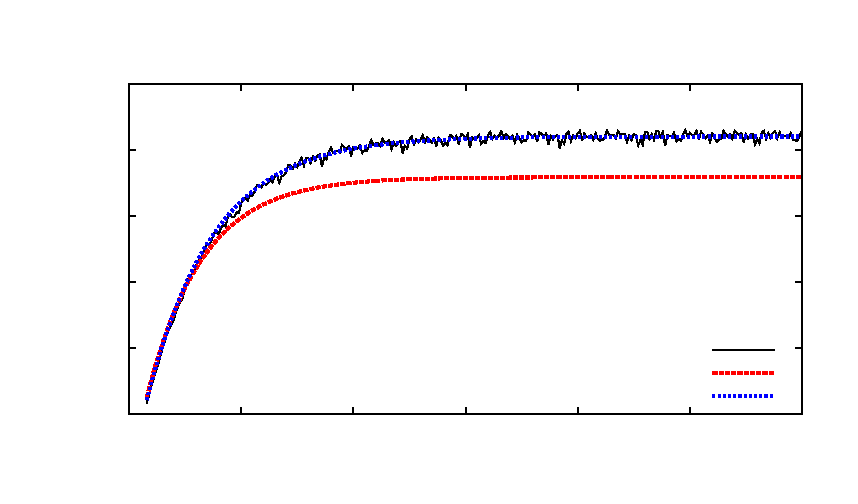
\includegraphics{../images/stepOutput}}%
    \gplfronttext
  \end{picture}%
\endgroup

    \caption{entrada degrau 1.5V}
    \label{fig:step}
    \end{subfigure}
    
  \begin{subfigure}{\linewidth}    
    % GNUPLOT: LaTeX picture with Postscript
\begingroup
  \makeatletter
  \providecommand\color[2][]{%
    \GenericError{(gnuplot) \space\space\space\@spaces}{%
      Package color not loaded in conjunction with
      terminal option `colourtext'%
    }{See the gnuplot documentation for explanation.%
    }{Either use 'blacktext' in gnuplot or load the package
      color.sty in LaTeX.}%
    \renewcommand\color[2][]{}%
  }%
  \providecommand\includegraphics[2][]{%
    \GenericError{(gnuplot) \space\space\space\@spaces}{%
      Package graphicx or graphics not loaded%
    }{See the gnuplot documentation for explanation.%
    }{The gnuplot epslatex terminal needs graphicx.sty or graphics.sty.}%
    \renewcommand\includegraphics[2][]{}%
  }%
  \providecommand\rotatebox[2]{#2}%
  \@ifundefined{ifGPcolor}{%
    \newif\ifGPcolor
    \GPcolorfalse
  }{}%
  \@ifundefined{ifGPblacktext}{%
    \newif\ifGPblacktext
    \GPblacktexttrue
  }{}%
  % define a \g@addto@macro without @ in the name:
  \let\gplgaddtomacro\g@addto@macro
  % define empty templates for all commands taking text:
  \gdef\gplbacktext{}%
  \gdef\gplfronttext{}%
  \makeatother
  \ifGPblacktext
    % no textcolor at all
    \def\colorrgb#1{}%
    \def\colorgray#1{}%
  \else
    % gray or color?
    \ifGPcolor
      \def\colorrgb#1{\color[rgb]{#1}}%
      \def\colorgray#1{\color[gray]{#1}}%
      \expandafter\def\csname LTw\endcsname{\color{white}}%
      \expandafter\def\csname LTb\endcsname{\color{black}}%
      \expandafter\def\csname LTa\endcsname{\color{black}}%
      \expandafter\def\csname LT0\endcsname{\color[rgb]{1,0,0}}%
      \expandafter\def\csname LT1\endcsname{\color[rgb]{0,1,0}}%
      \expandafter\def\csname LT2\endcsname{\color[rgb]{0,0,1}}%
      \expandafter\def\csname LT3\endcsname{\color[rgb]{1,0,1}}%
      \expandafter\def\csname LT4\endcsname{\color[rgb]{0,1,1}}%
      \expandafter\def\csname LT5\endcsname{\color[rgb]{1,1,0}}%
      \expandafter\def\csname LT6\endcsname{\color[rgb]{0,0,0}}%
      \expandafter\def\csname LT7\endcsname{\color[rgb]{1,0.3,0}}%
      \expandafter\def\csname LT8\endcsname{\color[rgb]{0.5,0.5,0.5}}%
    \else
      % gray
      \def\colorrgb#1{\color{black}}%
      \def\colorgray#1{\color[gray]{#1}}%
      \expandafter\def\csname LTw\endcsname{\color{white}}%
      \expandafter\def\csname LTb\endcsname{\color{black}}%
      \expandafter\def\csname LTa\endcsname{\color{black}}%
      \expandafter\def\csname LT0\endcsname{\color{black}}%
      \expandafter\def\csname LT1\endcsname{\color{black}}%
      \expandafter\def\csname LT2\endcsname{\color{black}}%
      \expandafter\def\csname LT3\endcsname{\color{black}}%
      \expandafter\def\csname LT4\endcsname{\color{black}}%
      \expandafter\def\csname LT5\endcsname{\color{black}}%
      \expandafter\def\csname LT6\endcsname{\color{black}}%
      \expandafter\def\csname LT7\endcsname{\color{black}}%
      \expandafter\def\csname LT8\endcsname{\color{black}}%
    \fi
  \fi
  \setlength{\unitlength}{0.0500bp}%
  \begin{picture}(7936.00,4534.00)%
    \gplgaddtomacro\gplbacktext{%
      \csname LTb\endcsname%
      \put(682,1364){\makebox(0,0)[r]{\strut{}-3}}%
      \put(682,1782){\makebox(0,0)[r]{\strut{}-2}}%
      \put(682,2200){\makebox(0,0)[r]{\strut{}-1}}%
      \put(682,2619){\makebox(0,0)[r]{\strut{} 0}}%
      \put(682,3037){\makebox(0,0)[r]{\strut{} 1}}%
      \put(682,3455){\makebox(0,0)[r]{\strut{} 2}}%
      \put(682,3873){\makebox(0,0)[r]{\strut{} 3}}%
      \put(814,1144){\makebox(0,0){\strut{} 0}}%
      \put(1487,1144){\makebox(0,0){\strut{} 1}}%
      \put(2159,1144){\makebox(0,0){\strut{} 2}}%
      \put(2832,1144){\makebox(0,0){\strut{} 3}}%
      \put(3504,1144){\makebox(0,0){\strut{} 4}}%
      \put(4177,1144){\makebox(0,0){\strut{} 5}}%
      \put(4849,1144){\makebox(0,0){\strut{} 6}}%
      \put(5522,1144){\makebox(0,0){\strut{} 7}}%
      \put(6194,1144){\makebox(0,0){\strut{} 8}}%
      \put(6867,1144){\makebox(0,0){\strut{} 9}}%
      \put(7539,1144){\makebox(0,0){\strut{} 10}}%
      \put(176,2618){\rotatebox{-270}{\makebox(0,0){\strut{}amplitude(m/s)}}}%
      \put(4176,814){\makebox(0,0){\strut{}tempo(s)}}%
      \put(4176,4203){\makebox(0,0){\strut{}Planta servo angular : reposta a onda quadrada}}%
    }%
    \gplgaddtomacro\gplfronttext{%
      \csname LTb\endcsname%
      \put(3321,393){\makebox(0,0)[r]{\strut{}saída experimental}}%
      \csname LTb\endcsname%
      \put(3321,173){\makebox(0,0)[r]{\strut{}modelo experimental}}%
      \csname LTb\endcsname%
      \put(6684,393){\makebox(0,0)[r]{\strut{}modelo teórico}}%
    }%
    \gplbacktext
    \put(0,0){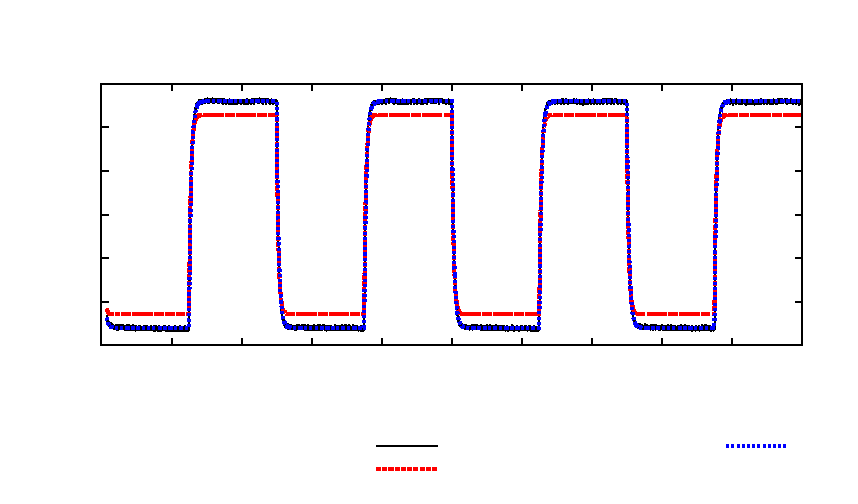
\includegraphics{../images/QuadradaOutput}}%
    \gplfronttext
  \end{picture}%
\endgroup

    \caption{entrada quadrada}
    \label{fig:quadrada}
 \end{subfigure}
\end{figure}
\FloatBarrier


%@@@@@@@@@@@@@@@@@@@@@@@@@@@@@@@@@@@@@@@@@@@
%@@@@@@@@@@@@@@       Análise         @@@@@@@@@@@@@@@@@@@@@@
%@@@@@@@@@@@@@@@@@@@@@@@@@@@@@@@@@@@@@@@@@@@@


\section{Discussão}
\subsection{Questão 1}
\paragraph{} Os resultados são mostrados nos gráficos \ref{fig:step} e
\ref{fig:quadrada}. Notamos que em ambos os gráficos o modelo obtido apresenta
resposta de menor amplitude que a resposta real. O motivo dessa discrepância
não é claro, mas origens desta podem se encontrar nas simplificações adotadas
na formulação do modelo teórico e na natureza imprecisa da formulação do atrito
e perca de potência na transmissão de engrenagens. Apesar dessa diferença no
valor final, podemos dizer que que ambas as resposta, teórica e experimental,
apresentam comportamento de primeira ordem, mostrando que o modelo adotado é
adequado para análise.
\subsection{Questão 2}
\paragraph{} Notamos que a resposta próximo do valor estacionário difere um
pouco do comportamento previsto pois oscilações significativas são
perceptíveis. Para tempos elevados, o valor parece oscilar em torno de um
valor fixo, atingindo momentaneamente valores superiores e inferiores a este. 
A resposta teórica nos diz que a resposta próxima do regime permanente deveria
ser no sentido de se aproximar de um valor constante, mas sempre inferiormente
a este, nunca o superando. Origens desse fenômeno podem se encontrar na própria
medida da velocidade, uma vez que os erros aleatórios envolvidos em todo
processo de medida geram essa oscilação de natureza gaussiana.

\subsection{Questão 3}
\paragraph{} Como visto na introdução, na fórmula \ref{eq:leEq}, a determinação
dos parâmetros envolve a medida do valor final da resposta experimental no
gráfico \ref{fig:step}. Uma vez que a resposta experimental não atinge de fato
um valor final, em vez disso, oscila em torno de um valor, foi necessário
contornar esse problema ao tomar como valor final a média dos últimos 50 pontos
obtidos. Uma vez que a matriz obtida da simulação com os dados abrangia cerca
de 300 instantes de tempo esse valor de 50 dados parece adequado para uma
estimativa do real valor final.
%@@@@@@@@@@@@@@@@@@@@@@@@@@@@@@@@@@@@@@@@@@@@@
%@@@@@@@@@@@@@@       Conclusão         @@@@@@@@@@@@@@@@@@@@@@
%@@@@@@@@@@@@@@@@@@@@@@@@@@@@@@@@@@@@@@@@@@@@@

\newpage
\section{Conclusão}
\paragraph{} O experimento permitiu obter a função de transferência 
de uma planta a partir do modelo teórico e da medição de parâmetros 
na resposta temporal. Notou-se que a função de transferência obtida 
não se comportou exatamente como o sistema em resposta ao degrau e à 
entrada quadrada, ficando a resposta teórica sempre abaixo da 
resposta experimental. Possivelmente essas falhas se devam a 
imperfeições e simplificações feitas na análise teórica, de forma que 
a função de transferência real não possui exatamente a fórmula 
suposta para ela. Além disso, a resposta ao degrau apresentou comportamento
oscilatório para altas constantes de tempo, de modo que foi necessário tomar
uma média dos valores finais para se obter uma estimativa do valor em regime
permanente.

%@@@@@@@@@@@@@@@@@@@@@@@@@@@@@@@@@@@@@@@@@@@@@@
%@@@@@@@@@@@@@@       REFERÊNCIAS     @@@@@@@@@@@@@@@@@@@@@@
%@@@@@@@@@@@@@@@@@@@@@@@@@@@@@@@@@@@@@@@@@@@@@@
\begin{thebibliography}{9}    
	 \bibitem{ADL-NISE}
  		Nise, N.S.
  		\emph{Engenharia de Sistemas de Controle}
 		 5ª ed.
		LTC, 2009.

	 \bibitem{ADL-OGATA}
  		Ogata, K.
  		\emph{Moder Control Engeeniring}
 		 5ª ed.
		Pearson, 2010.
	 
\end{thebibliography}
\end{document}
